\documentclass[11pt, oneside]{article}   	% use "amsart" instead of "article" for AMSLaTeX format
\usepackage{geometry}                		% See geometry.pdf to learn the layout options. There are lots.
\geometry{letterpaper}                   		% ... or a4paper or a5paper or ... 
%\geometry{landscape}                		% Activate for for rotated page geometry
%\usepackage[parfill]{parskip}    		% Activate to begin paragraphs with an empty line rather than an indent
\usepackage{graphicx}				% Use pdf, png, jpg, or eps§ with pdflatex; use eps in DVI mode
								% TeX will automatically convert eps --> pdf in pdflatex		
\usepackage{amssymb}
\usepackage{amsmath}
\usepackage{parskip}
\usepackage{color}
\usepackage{hyperref}

\title{Functions of a complex variable:  differentiation}
%\author{The Author}
%\section{}
%\subsection*{}
\date{}							% Activate to display a given date or no date

\graphicspath{{/Users/telliott_admin/Dropbox/Tex/png/}}
% \begin{center} 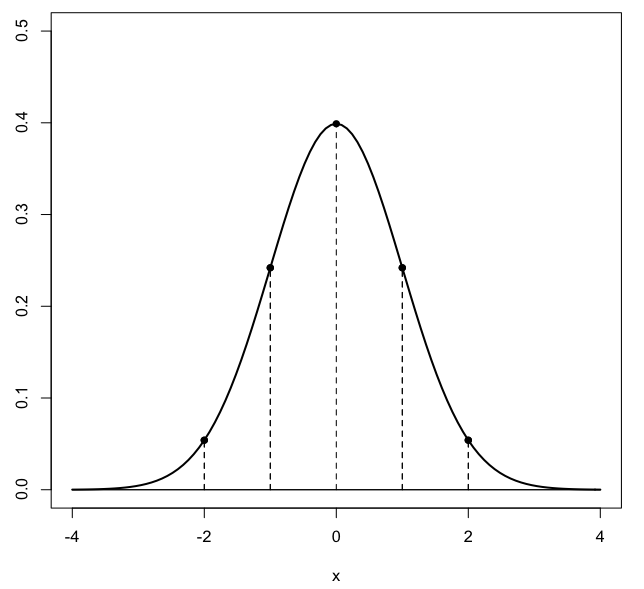
\includegraphics [scale=0.4] {gauss3.png} \end{center}
\begin{document}
\maketitle
\Large
This section contains a general discussion of differentiation of complex functions, which gives us a first glimpse of the important Cauchy-Riemann conditions and justifies our first formula for calculating the derivative
\[ f'(z) = u_x + i v_x \]

As an example of its use, consider the complex exponential
\[ f(z) = e^z \]
If we write $z = x + iy$ then
\[ f(z) = e^{x + iy} \]
\[ = e^x e^{iy} \]
and (from Euler):
\[ = e^x (\cos y + i \sin y) \]
Using the formula, it can be shown easily that the derivative is the same as the function itself, just as for the case of real numbers.
\[ u(x,y) = e^x \cos y \]
\[ u_x = e^x \cos y = u \]
\[ v(x,y) = e^x \sin y \]
\[ v_x = e^x \sin y = v \]
Hence
\[f'(z) = u + iv = z \]

\subsection*{definition}
We define the derivative $f'(z)$ of a complex function $f(z)$ similarly to the derivative of a real function.  We say that:
\[ f'(z) = \lim_{w \rightarrow z} \ \frac{f(w) - f(z)}{w-z} \]
Alternatively, with $\Delta$ notation, we might write:
\[ f'(z) = \lim_{\Delta z \rightarrow 0} \ \frac{f(z + \Delta z) - f(z)}{\Delta z} \]

A crucial point is that the limit is over \emph{all} possible ways of approaching $z$ in the Argand plane.  

If the limit exists, the function $f$ is called differentiable and $f'(z)$ is the derivative.
Consider
\[ f(z) = u(x,y) + i v(x,y) \]
Then
\[ f'(z) = \frac{f(z + \Delta z) - f(z)}{\Delta z} \]
\[ = \frac{u(x + \Delta x, y + \Delta y) + i v (x + \Delta x, y + \Delta y) - u(x,y) - i v(x,y)}{\Delta x + i \Delta y} \]

\subsection*{fixed y}
Looking at the special path along the $x$-axis where $\Delta y = 0$ we obtain
\[ f'(z) = \frac{u(x + \Delta x, y) + i v (x + \Delta x, y) - u(x,y) - i v(x,y)}{\Delta x} \]
Rearrange the numerator
\[ = \frac{u(x + \Delta x, y) - u(x,y)}{\Delta x} + \frac{i v (x + \Delta x, y) - i v(x,y)}{\Delta x} \]
The first term is
\[ u_x = \frac{\partial u}{\partial x} \]
and the second term is 
\[ i v_x \]
Hence we conclude that
\[ f'(z) = u_x + i v_x \]

\subsection*{fixed x}
Now look at the special path along the $y$-axis where $\Delta x = 0$:
\[ f'(z) = \frac{u(x, y + \Delta y) + i v (x, y + \Delta y) - u(x,y) - i v(x,y)}{i \Delta y} \]
Rearrange the numerator
\[ = \frac{u(x, y + \Delta y) - u(x,y)}{i \Delta y} + \frac{i v (x, y + \Delta y) - i v(x,y)}{i \Delta y} \]
\[ = \frac{1}{i} u_y + v_y \]
Recall that $1/i = -i$
\[ f'(z) = v_y - i u_y \]

\subsection*{Putting it together}
We require that the limit be the same regardless of the direction of approach to $z$, so in particular, these two expressions for the difference quotient must be equal:
\[ f'(z) = u_x + i v_x = - i u_y + v_y \]
Both the real and the imaginary parts must be equal so
\[ u_x  = v_y \]
\[ u_y = - v_x \]
And, as we said at the beginning, in looking at various complex functions we can use this fact:
\[ f'(z) = u_x + i v_x \]
In other words
\[ \frac{df}{dz} = \frac{\partial f}{\partial x} \]
and since
\[ u_x + i v_x = v_y - i u_y \]
\[ \frac{df}{dz} = -i \frac{\partial f}{\partial y} \]

\subsection*{more}
When we get to integration in a later section we will find that we integrate complex functions as line integrals along a specified curve (perhaps a circle centered on the origin or on a point $z_0$).  This curve relates the values of $x$ and $y$ and allows us to parametrize either $y$ in terms of $x$ or more generally, both $x$ and $y$ in terms of a single real variable or parameter $t$.

When we have a function of such a variable like
\[ f(t) = u(t) + i v(t) \]
then the derivative is defined to be
\[ f'(t) = u'(t) + i v'(t) \]
where $u$ and $v$ are real-valued functions of a single real variable and so follow the standard rules from introductory calculus.  In particular if
\[ w(t) = z_0 f(t) \]
then
\[ w'(t) = z_0 f'(t) \]
We can show this by using a little algebra:
\[ \frac{d}{dt} \ z_0 f(t) = \ [ \ (x_0 + i y_0) (u + iv) \ ]' \]
\[ = \ [ \ (x_0 u - y_0 v) + i (y_0 u + x_0 v) \ ]' \]
\[ = (x_0 u - y_0 v)' + i (y_0 u + x_0 v)' \]
\[ = (x_0 u' - y_0 v') + i (y_0 u' + x_0 v') \]
\[ = (x_0 + i y_0)(u' + iv') \]
\[ = z_0 \frac{d}{dt} \ f(t) \]
Thus
\[ \frac{d}{dt} \ z_0 f(t) = z_0 \frac{d}{dt} \ f(t) \]

Another expected result is
\[ \frac{d}{dt} \ e^{z_0 t} = z_0 e^{z_0 t} \]
where $z_0$ is a complex constant and $t$ is a real variable.

To do this one, refer to the definition
\[ f'(t) = u'(t) + i v'(t) \]
and now we need to break up the exponential into its real and imaginary parts.  

We write as we did above
\[ e^z = e^{x + iy} \]
\[ = e^x \ e^{iy} \]
by Euler's equation
\[ = e^x \ (\cos y + i \sin y) \]
\[ = e^x \cos y + i e^x \sin y \]

For the exponential with a constant we have
\[ e^{z_0 t} = e^{(x_0 + iy_0) t} \]
\[ = e^{x_0t} \ e^{i y_0 t} \]
\[ = e^{x_0t} \ (\cos y_0 t + i \sin y_0 t) \]
\[ = e^{x_0t} \cos y_0 t + i e^{x_0t} \ \sin y_0 t \]

Using the definition above we get that the derivative is
\[ \frac{d}{dt} \ e^{z_0 t} = x_0 e^{x_0t} \cos y_0 t  - y_0 e^{x_0t} \sin y_0 t + i(x_0 e^{x_0t} \sin y_0 t + y_0 e^{x_0t} \cos y_0 t) \]
\[ = x_0(e^{x_0t} \cos y_0 t + i e^{x_0 t} \sin y_0 t) + i y_0(e^{x_0t} \cos y_0 t + i e^{x_0 t} \sin y_0 t) \]
\[ = x_0 e^{z_0 t} + i y_0 e^{z_0 t} \]
\[ = (x_0 + iy_0) e^{z_0 t} \]
\[ = z_0 e^{z_0 t} \]
which is what we needed to prove.


\end{document}  